%% Copyright 2017 Eric Griffis <dedbox@gmail.com>
%% 
%% Licensed under the Apache License, Version 2.0 (the "License");
%% you may not use this file except in compliance with the License.
%% You may obtain a copy of the License at
%% 
%% http://www.apache.org/licenses/LICENSE-2.0
%% 
%% Unless required by applicable law or agreed to in writing, software
%% distributed under the License is distributed on an "AS IS" BASIS,
%% WITHOUT WARRANTIES OR CONDITIONS OF ANY KIND, either express or implied.
%% See the License for the specific language governing permissions and
%% limitations under the License.

\documentclass[letterpaper,12pt,openany]{report}

\newcommand{\NetTwo}{\texttt{net2}}

% title page
\title{\NetTwo  \\ Technical Specification}
\author{Eric Griffis \\ dedbox@gmail.com}
\date{\today}
\usepackage[firstpage]{draftwatermark}
\SetWatermarkScale{7}

% general includes
\usepackage[margin=1in]{geometry}
\usepackage[parfill]{parskip}
\usepackage{color}
\usepackage{amsmath,amssymb}
\usepackage{upgreek}
\usepackage{semantic}
\usepackage{mathpartir}
\usepackage{colonequals}
\usepackage{array}
\usepackage{fancyvrb}

% debugging and drafting
\newenvironment{xxx}{\color{red}}{}
\newcommand{\XXX}[1]{\begin{xxx}#1\end{xxx}}

% diagrams
\usepackage{tikz}

% sets
\DeclareMathOperator{\As}{\ensuremath{\mathcal{A}}}
\DeclareMathOperator{\Bs}{\ensuremath{\mathcal{B}}}
\DeclareMathOperator{\Cs}{\ensuremath{\mathcal{C}}}
\DeclareMathOperator{\Ds}{\ensuremath{\mathcal{D}}}
\DeclareMathOperator{\Ls}{\ensuremath{\mathcal{L}}}
\DeclareMathOperator{\Is}{\ensuremath{\mathcal{I}}}
\DeclareMathOperator{\Os}{\ensuremath{\mathcal{O}}}
\DeclareMathOperator{\Ps}{\ensuremath{\mathcal{P}}}
\DeclareMathOperator{\Qs}{\ensuremath{\mathcal{Q}}}
\DeclareMathOperator{\Rs}{\ensuremath{\mathcal{R}}}
\DeclareMathOperator{\Ss}{\ensuremath{\mathcal{S}}}
\DeclareMathOperator{\Ts}{\ensuremath{\mathcal{T}}}
\DeclareMathOperator{\Us}{\ensuremath{\mathcal{U}}}
\DeclareMathOperator{\Void}{\ensuremath{\varnothing}}

% operations
\DeclareMathOperator{\Scheme}{\textsf{scheme}}
\DeclareMathOperator{\Authority}{\textsf{authority}}
\DeclareMathOperator{\Path}{\textsf{path}}
\DeclareMathOperator{\Query}{\textsf{query}}

\DeclareMathOperator{\Accept}{\textsf{accept}}
\DeclareMathOperator{\Connect}{\textsf{connect}}
\DeclareMathOperator{\Listen}{\textsf{listen}}
\DeclareMathOperator{\Receive}{\textsf{receive}}
\DeclareMathOperator{\Release}{\textsf{release}}
\DeclareMathOperator{\Send}{\textsf{send}}

% variables
\newcommand{\Lx}{\text{L}}
\newcommand{\Tx}{\text{T}}
\newcommand{\Dx}{\text{D}}
\newcommand{\T}{\uptau}

% helpers
\DeclareMathOperator{\Accepter}{accepter}
\DeclareMathOperator{\Connector}{connector}
\DeclareMathOperator{\Listener}{listener}
\DeclareMathOperator{\Receiver}{receiver}
\DeclareMathOperator{\Sender}{sender}

% symbols
\mathlig{|-->}{\mapsto}
\mathlig{-->}{\leadsto}
\mathlig{=>}{\Downarrow}
\mathlig{->}{\rightarrow}
\mathlig{|-}{\vdash}
\mathlig{**}{\times}
\mathlig{<}{\langle}
\mathlig{>}{\rangle}

% layout
\newcolumntype{L}{>{$}l<{$}}
\newcolumntype{C}{>{$}c<{$}}
\newcolumntype{R}{>{$}r<{$}}
\newcolumntype{+}{@{~}}
\newcolumntype{^}{@{\extracolsep{\fill}}}
\newcolumntype{=}[1]{@{$#1$}}

% syntax
\newenvironment{Grammar}{
  \begin{tabular}[t]{l}
    \begin{minipage}[t]{.45\linewidth}
      \begin{tabular*}{\linewidth}{L+C+L^r}
}{
      \end{tabular*}
    \end{minipage}
  \end{tabular}
}

% semantics
\newcommand{\Rule}[1]{\text{\textsc{#1}}}
\newcommand{\Infer}[3][]{\inferrule{#2}{#3}~\Rule{#1}}

% back matter
\newcommand{\BackChapter}[1]{\chapter*{#1}\addcontentsline{toc}{chapter}{#1}}

% glossary
\newcommand{\GlossaryItem}[2]{
  \paragraph{#1} #2\vspace{-1ex}
}

%%%%%%%%%%%%%%%%%%%%%%%%%%%%%%%%%%%%%%%%%%%%%%%%%%%%%%%%%%%%%%%%%%%%%%%%%%%%%%%%
%%%%%%%%%%%%%%%%%%%%%%%%%%%%%%%%%  REFERENCES  %%%%%%%%%%%%%%%%%%%%%%%%%%%%%%%%%
%%%%%%%%%%%%%%%%%%%%%%%%%%%%%%%%%%%%%%%%%%%%%%%%%%%%%%%%%%%%%%%%%%%%%%%%%%%%%%%%

\usepackage{natbib}
\usepackage{tocbibind}
\renewcommand{\bibname}{References}

\begin{filecontents*}{references.bib}
@article{berners2014rfc,
  title={Rfc 3986, uniform resource identifier (uri): Generic syntax, 2005},
  author={Berners-Lee, Tim and Fielding, Roy and Masinter, Larry},
  journal={URL: http://www. faqs. org/rfcs/rfc3986. HTML},
  year={2014}
}
\end{filecontents*}

%%%%%%%%%%%%%%%%%%%%%%%%%%%%%%%%%%%%%%%%%%%%%%%%%%%%%%%%%%%%%%%%%%%%%%%%%%%%%%%%
%%%%%%%%%%%%%%%%%%%%%%%%%%%%%%%%%%  DOCUMENT  %%%%%%%%%%%%%%%%%%%%%%%%%%%%%%%%%%
%%%%%%%%%%%%%%%%%%%%%%%%%%%%%%%%%%%%%%%%%%%%%%%%%%%%%%%%%%%%%%%%%%%%%%%%%%%%%%%%

\begin{document}

%%%%%%%%%%%%%%%%%%%%%%%%%%%%%%%%%%%%%%%%%%%%%%%%%%%%%%%%%%%%%%%%%%%%%%%%%%%%%%%%
%%%%%%%%%%%%%%%%%%%%%%%%%%%%%%%%  FRONT MATTER  %%%%%%%%%%%%%%%%%%%%%%%%%%%%%%%%
%%%%%%%%%%%%%%%%%%%%%%%%%%%%%%%%%%%%%%%%%%%%%%%%%%%%%%%%%%%%%%%%%%%%%%%%%%%%%%%%

\pagenumbering{roman}

\maketitle

\begin{abstract}
  This is a technical specification for {\NetTwo}, a networking abstraction
  for URL-addressable agents communicating via byte streams. Its purpose is to
  drive the engineering design process.
\end{abstract}

\tableofcontents

\listoffigures

%%%%%%%%%%%%%%%%%%%%%%%%%%%%%%%%%%%%%%%%%%%%%%%%%%%%%%%%%%%%%%%%%%%%%%%%%%%%%%%%
%%%%%%%%%%%%%%%%%%%%%%%%%%%%%%%%  BODY MATTER  %%%%%%%%%%%%%%%%%%%%%%%%%%%%%%%%%
%%%%%%%%%%%%%%%%%%%%%%%%%%%%%%%%%%%%%%%%%%%%%%%%%%%%%%%%%%%%%%%%%%%%%%%%%%%%%%%%

\clearpage
\pagenumbering{arabic}
\setcounter{page}{1}
\pagestyle{plain}

%%%%%%%%%%%%%%%%%%%%%%%%%%%%%%%%%%  CHAPTER  %%%%%%%%%%%%%%%%%%%%%%%%%%%%%%%%%%%

\chapter{Introduction}
\label{cha:introduction}

This report defines an abstract model for {\NetTwo}.

\begin{figure}
  \centering
  
  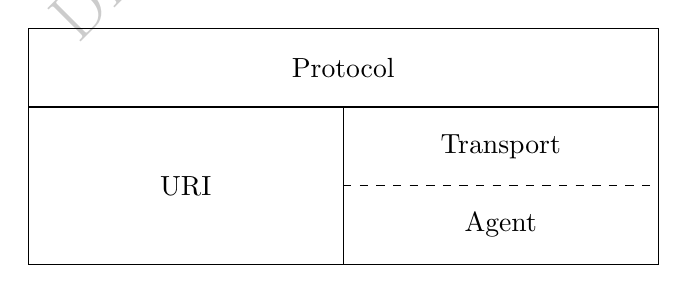
\begin{tikzpicture}[y=-1cm]
    \node at (0, 1) {Protocol};
    \node at (-2, 2.5) {URI};
    \node at (2, 2) {Transport};
    \node at (2, 3) {Agent};
    \draw (-4, 0.5) -- (4, 0.5) -- (4, 3.5) -- (-4, 3.5) -- cycle;
    \draw (-4, 1.5) -- (4, 1.5);
    \draw (0, 1.5) -- (0, 3.5);
    \draw (0, 2.5) -- (4, 2.5) [dashed];
  \end{tikzpicture}

  \caption{The {\NetTwo} API stack}
  \label{fig:net2-api-stack}
\end{figure}

%%%%%%%%%%%%%%%%%%%%%%%%%%%%%%%%%%  CHAPTER  %%%%%%%%%%%%%%%%%%%%%%%%%%%%%%%%%%

\chapter{URI}
\label{cha:uri}

\begin{xxx}
  \begin{itemize}
  \item Explain how URIs work in {\NetTwo}.

    ``A URI has several parts. The authority defines \emph{who} you are
    talking to. The scheme defines \emph{how} you talk to them. The path and
    query define \emph{what resource} you're talking to them about.''

  \item We roll our own URI sub-system.
  \end{itemize}
\end{xxx}

\begin{mathpar}
  \Ss = \text{schemes}

  \As = \text{authorities}

  \Ps = \text{paths}

  \Qs = \text{queries}
\end{mathpar}

\begin{mathpar}
  \Scheme : \Us -> \Ss

  \Authority : \Us -> \As
  
  \Path : \Us -> \Ps

  \Query : \Us -> \Qs
\end{mathpar}

%%%%%%%%%%%%%%%%%%%%%%%%%%%%%%%%%%  CHAPTER  %%%%%%%%%%%%%%%%%%%%%%%%%%%%%%%%%%

\chapter{Transport}
\label{cha:transport}

A \emph{byte stream} is a one-way communications channel. A \emph{connection}
is a pair of opposing byte streams.

\section{Primitive types}
\label{sec:transport-primitive-types}

\subsection*{References}

\begin{mathpar}
  \Ls = \text{listeners}

  \Ts = \text{transports}

  \Rs = \Ls \cup \Ts
\end{mathpar}

A \emph{reference} is an opaque token that represents a portion of run-time
state. A listener represents a connection request queue. A transport
represents a connection.

\subsection*{Ports}

\begin{mathpar}
  \Is = \text{input ports}

  \Os = \text{output ports}
\end{mathpar}

A \emph{port} is a host platform object that represents one end of a byte
stream. Ports come in pairs---an input port and an output port. An output port
sends bytes to the byte stream. An input port receives bytes from the byte
stream.

\subsection*{Literals}

\begin{mathpar}
  \Bs = \text{byte arrays}

  \Void = \text{void}
\end{mathpar}

A \emph{literal} is a fixed unit of data. A byte array is a unit of data
exchange. The void literal is returned by operations with a side effect and no
useful result.

\section{Dictionaries}
\label{sec:transport-dictionaries}

\begin{mathpar}
  \Ds = \{\Rs -> *\}
\end{mathpar}

A \emph{dictionary} is an associative array. Dictionaries associate references
to some underlying data. Associations can be added, removed, or looked up.

\begin{figure}
  \centering
  \begin{tabular}{ll}
    $[k |--> v]\Dx$ & associate $k$ with $v$ in $\Dx$. \\
    $\Dx \setminus \{k |--> \cdot\}$ & remove from $\Dx$ the association keyed by $k$. \\
    $\Dx(k)$ & lookup $k$ in $\Dx$. \\
  \end{tabular}
  
  \caption{Dictionary notation}
  \label{fig:dictionary-notation}
\end{figure}

\section{The run-time state}
\label{sec:transport-run-time-state}

\begin{mathpar}
  \Lx : \Ls -> \As

  \Tx : \Ts -> \As ** \As ** \Is ** \Os
\end{mathpar}

The run-time state is a set of dictionaries. All side effects occur during
operations on dictionaries in the run-time state.

$\Lx$ records the addresses of listeners. Given listener $\ell$ and local
authority authority $a_L$, the host platform queues requests to connect to
$a_L$ under $\ell$ for as long as $\Lx(\ell) = a_L$.

$\Tx$ records the addresses and ports of established connections. Given
transport $\T$, addresses $a_L, a_R$, and ports $p_I, p_O$, the host platform
establishes a connection between local authority $a_L$ and remote authority
$a_R$ for as long as $\Tx(\T) = (a_L, a_R, p_I, p_O)$. Updating $p_I$ or $p_O$
will exchange bytes over the connection.

\section{The Agent API}
\label{sec:transport-agent-api}

A registered name driver implements the operations defined in this section.

\begin{mathpar}
  \Listener : \As -> \Ls

  \Listener(a_L) = \ell
\end{mathpar}

Creates a reference $\ell$ to a connection request queue associated with local
authority $a_L$.

\begin{mathpar}
  \Accepter : \Ls -> \Ts ** \As ** \Is ** \Os

  \Accepter(\ell) = <\T, a_R, p_I, p_O>
\end{mathpar}

Creates a reference $\T$ to a connection request from remote authority $a_R$
queued under listener $\ell$. Opens ports $p_I, p_O$ for exchanging bytes over
the connection.

\begin{mathpar}
  \Connector : \As -> \Ts ** \As ** \Is ** \Os

  \Connector(a_R) = <\T, a_L, p_I, p_O>
\end{mathpar}

Creates a reference $\T$ to a connection from local authority $a_L$ to remote
authority $a_R$. Opens ports $p_I, p_O$ for exchanging bytes over the
connection.

\begin{mathpar}
  \Sender : \Bs ** \Os -> \Os

  \Sender(b, p_O) = p_O'
\end{mathpar}

Creates a port update $p_O'$ that writes byte array $b$ to port $p_O$.

\begin{mathpar}
  \Receiver : \Is -> \Bs ** \Is

  \Receiver(p_I) = <b, p_I'>
\end{mathpar}

Creates a port update $p_I'$ that reads byte array $b$ from port $p_I$.

\section{Creating and destroying connections}
\label{sec:transport-creat-destr-conn}

\begin{figure}
  \centering

  \begin{Grammar}
    t
    &::=& \Listen(t) & bind authority \\
    & | & \Accept(t) & accept connection \\
    & | & \Connect(t) & connect to authority \\
    & | & \Release(t) & unbind / disconnect \\
    & | & \Send(t, t) & send bytes \\
    & | & \Receive(t) & receive bytes \\
  \end{Grammar}
  \hfill
  \begin{Grammar}
    v
    &::=& a & authority \\
    & | & b & byte array \\
    & | & \ell & listener \\
    & | & \T & transport \\
    & | & u & URI \\
    & | & \Void & void \\
  \end{Grammar}
  
  \caption{Transport syntax}
  \label{fig:core-syntax}
\end{figure}

\begin{mathpar}
  \Listen : \As -> \Ls

  \Listen(a_L) = \ell

  \Infer[Lsn]{
    \Listener(a_L) = \ell
  }{
    \Lx |- \Listen(a_L) --> [\ell |--> a_L]\Lx |- \ell
  }
\end{mathpar}

Creates a listener $\ell$ on local authority $a_L$.

\begin{mathpar}
  \Accept : \Ls -> \Ts

  \Accept(\ell) = \T

  \Infer[Acc]{
    \Lx(\ell) = u_L \and \Accepter(\ell) = <\T, a_R, p_I, p_O>
  }{
    \Tx |- \Accept(\ell) --> [\T |--> <a_L, a_R, p_I, p_O>]\Tx |- \T
  }
\end{mathpar}

Accepts a transport $\T$ from listener $\ell$.

\begin{mathpar}
  \Connect : \As -> \Ts

  \Connect(a) = \T

  \Infer[Con]{
    \Connector(a_R) = <\T, a_L, p_I, p_O>
  }{
    \Tx |- \Connect(a_R) --> [\T |--> <a_L, a_R, p_I, p_O>]\Tx |- \T
  }
\end{mathpar}

Connects a transport $\T$ from local authority $a_L$ to remote authority
$a_R$.

\begin{mathpar}
  \Release : \Rs -> \Void

  \Release(r) = \Void

  \Infer[Rls]{
  }{
    \Lx |- \Release(r) --> \Lx \setminus \{r |--> \cdot\} |- \Void
  }
\end{mathpar}

Stops listening when $r$ is a listener. Closes the connection when $r$ is a
transport.

\section{Exchanging bytes}
\label{sec:transport-exchanging-bytes}

\begin{mathpar}
  \Send : \Bs ** \Ts -> \Void

  \Send(b, \T) = \Void

  \Infer[Snd]{
    \Tx(\T) = <a_L, a_R, p_I, p_O> \and \Sender(b, p_O) = p_O'
  }{
    \Tx |- \Send(b, \T) --> [\T |--> <a_L, a_R, p_I, p_O'>]\Tx |- \Void
  }
\end{mathpar}
  
Sends byte array $b$ over transport $\T$.

\begin{mathpar}
  \Receive : \Ts -> \Bs

  \Receive(\T) = b

  \Infer[Rcv]{
    \Tx(\T) = <a_L, a_R, p_I, p_O> \and \Receiver(p_I) = <b, p_I'>
  }{
    \Tx |- \Receive(\T) --> [\T |--> <a_L, a_R, p_I', p_O>]\Tx |- b
  }
\end{mathpar}

Receives byte array $b$ over transport $\T$.

%%%%%%%%%%%%%%%%%%%%%%%%%%%%%%%%%%  CHAPTER  %%%%%%%%%%%%%%%%%%%%%%%%%%%%%%%%%%%

\chapter{Protocol}
\label{cha:protocol}

\section{Codecs}

\section{Messengers}

\section{Clients and servers}

%%%%%%%%%%%%%%%%%%%%%%%%%%%%%%%%%%%%%%%%%%%%%%%%%%%%%%%%%%%%%%%%%%%%%%%%%%%%%%%%
%%%%%%%%%%%%%%%%%%%%%%%%%%%%%%%%  BACK MATTER  %%%%%%%%%%%%%%%%%%%%%%%%%%%%%%%%%
%%%%%%%%%%%%%%%%%%%%%%%%%%%%%%%%%%%%%%%%%%%%%%%%%%%%%%%%%%%%%%%%%%%%%%%%%%%%%%%%

\appendix

\BackChapter{Glossary}
\label{cha:glossary}

\GlossaryItem{agent}{A URL-addressable process capable of exchanging bytes.}

\GlossaryItem{authority}{The authority component of a URI. This could be an IP
  address and port number, or other kinds of extensible
  registered~names~\cite{berners2014rfc}.}

\GlossaryItem{byte array}{A finite sequence of bytes.}

\GlossaryItem{byte stream}{A one-way communications channel.}

\GlossaryItem{connection}{A two-way communications channel.}

\GlossaryItem{connector}{A means of requesting a connection to another agent.}

\GlossaryItem{dictionary}{A binary relation between references and run-time
  state.}

\GlossaryItem{host platform}{The programming platform implementing {\NetTwo}.}

\GlossaryItem{input port}{A port that receives bytes.}

\GlossaryItem{listener}{A means of accepting connection requests from other
  agents.}

\GlossaryItem{output port}{A port that sends bytes.}

\GlossaryItem{port}{One end of a byte stream.}

\GlossaryItem{reference}{An opaque token that identifies a set of related
  objects.}

\GlossaryItem{scheme}{The scheme component of a URI.}

\GlossaryItem{transport}{A reliable, buffered, and ordered means of exchanging
  bytes with other agents.}

\GlossaryItem{URL}{A URI, as defined in RFC~3986~\cite{berners2014rfc}, that
  locates an agent.}

%%%%%%%%%%%%%%%%%%%%%%%%%%%%%%%%%%%%%%%%%%%%%%%%%%%%%%%%%%%%%%%%%%%%%%%%%%%%%%%%

\bibliographystyle{alpha}
\bibliography{references.bib} 
\label{cha:references}

\BackChapter{License}
\label{cha:license}

\VerbatimInput{LICENSE}

\end{document}
